\section{Introduction}

Phenology, the timing of seasonal biological phenomena, is a key aspect of plant and animal life.
It defines the timing and duration of growth and reproduction and thereby determines the ability to capture seasonally variable resources \citep{chuine2017process}.
%The study of plant and animal phenology has allowed for a better understanding of fundamental ecosystem processes such as biogeochemical cycles,
%trophic interactions, animal migrations, and the response of populations and communities to global climate change,
%as well as informing applications in agriculture, forestry, and public health such as varietal selection in plant and animal breeding, or integrated pest and disease management .

Phenological analyses often focus on the timing of particular events, such as the dates of peak plant flowering \citep{aono2008phenological}.%, the dates of egg laying in birds \cite{shutt2019environmental}, or the dates of first or peak appearance of butterflies \citep{roy2000phenology}.
However, for many biological phenomena exact dates of particular events are more difficult to observe than the state of the system itself.
For example, repeated but sparse survey visits may record whether a plant is in bud, flowering, or setting fruit, but not the exact dates when each of those stages was reached.
%Similarly, surveys may record the development stage of insects or amphibians, or the breeding or moult status of birds.
Such observations can be used to categorize an organism's state into discrete classes which usually follow natural ordering, e.g. from least to most developed. 
The resulting data can be described using ordinal regression models \cite{mccullagh1980regression,agresti2010analysis}.

I here replicate a number of ordinal regression models that were developed by \citet{dennis1986stochastic} and \citet{candy1991modeling} to describe insect phenology. 

\section{Data}
The models replicated in this study are fitted to a data set on the phenology of the western spruce budworm \emph{Choristoneura freemani} (Lepidoptera: Tortricidae), a defoliating moth that is widespread in western North America \citep{brookes1987western}. This data set was originally published in \citep{dennis1986stochastic} and is a subset of a larger budworm survey data set analysed in \citep{kemp1986stochastic}. The data consist of 12 sampling occassions at which counts of individual budworms in each of seven development stages (five larval instars, pupae, and adults) were recorded. The only available covariate is a measure of seasonal progression, the accumulated degree days calculated using a threshold of 5.5°C. \citet{candy1991modeling} noted an inconsistency in these data, namely that the reported total number of individuals did not correspond to the sum across the seven development stages for two of the sampling occasions. I therefore use the data set as it was republished in \citep{candy1990biology}, where numbers in each stage have been assumed correct and the totals for each sampling occasion were adjusted accordingly.

\section{Methods}
The statistical models replicated here are different types of ordinal regression models \citep{agresti2010analysis} all with the aim of predicting the proportion of an insect population in a particular development stage at any given given time. In particular, they represent three different parametrisations of the so-called cumulative model and one version of the so-called sequential model. A recent summary of the theory underlying these models is provided in \citep{burkner2019ordinal}.

The models generally assume that the development of an insect follows an unobservable stochastic process $S(t)$ consisting of accumulated increments of development over time $t$. As the amount of $S(t)$ increases, the insect passes through successive stages, delimited by moults, with the $j$th moult occuring when the development threshold $a_j$ is reached:

\begin{alignat*}{3}
  \mathrm{stage}\,1&:\qquad {}&   S(t) & \leq a_1 \\
  \mathrm{stage}\,2&:\qquad  a_1&< S(t) & \leq a_2 \\
  \vdots & &\vdots \\
  \mathrm{stage}\,r-1&:\qquad  a_{r-2}&< S(t) & \leq a_{r-1} \\
  \mathrm{stage}\,r&:\qquad  a_{r-1}&< S(t) 
\end{alignat*}

The $a_j$ values are typically unknown and must be estimated from the data.

\subsection{Cumulative model with constant variance }
If the cumulative number of individuals observed in stages 1 to $j$ is given by $m_{ij}=\sum_{k=1}^jn_{ik}$ then the ordinal regression model \citep{mccullagh1980regression} is specified by %TODO: tidy up indices r vs j to be consistent in enumerating the stages
\begin{alignat}{1}
\mathbf{E}(m_{ij})&=N_iPr(S(t) < \alpha_j), \qquad j = 1,\dots ,r\\
&=N_iG(\alpha_j + \beta z_i)
\end{alignat}
where $G$ is the cumulative probability density function of $S(t)$, $\alpha_j$ are ordered thresholds or cut-point parameters, $\beta$ is a vector of regression parameters and $z_i$ is a vector of predictor variables.
If the probability of an individual being in stage $j$ or earlier at time $t_i$ is $$\mu_{ij} = \mathbf{E}(m_{ij})/N_i$$ one can define $G^{-1}$ as the link function of a generalised linear model with the linear predictor $$\eta_{ij}=\alpha+\beta z_i$$. This ordinal regression model is commonly known as the cumulative model, and is applied to the budworm data in \citep{candy1991modeling} using the logit and complementary log-log link functions. In  both cases the parametrisation results in a constant variance for $S(t)$. \citet{candy1991modeling} reexpresses the model in terms of stage-specific counts $n_{ij}$  
\begin{equation}
\mathbf{E}(n_{ij})=N_i\{G(\alpha_j + \beta z_i) - G(\alpha_{j-1} + \beta z_i)\}
\label{eq:candy_cm_count_form}
\end{equation}
and fits it using a Poisson likelihood \citep{thompson1981composite}. No code is provided for this estimation procedure in the original paper, however, \citep{candy1990biology} provides a set of example macros for the software package \verb+GLIM+ \citep{aitkin1989statistical} which is no longer actively developed or distributed. I therefore created an R version of the estimation procedure which directly optimizes a Poisson log-likelihood for (\ref{eq:candy_cm_count_form}) using the \verb+optim+ function. The cumulative model is also implemented in various R packages, including in the \verb+vglm+ function in \verb+VGAM+ \citep{VGAM} and the \verb+clm+ function in \verb+ordinal+ \cite{ordinal} and I here make use of these to fit the model to the budworm data.

\subsection{Cumulative model with proportional variance}
\citet{dennis1986stochastic} proposed a different parameterisation of the ordinal model is based on assuming a logistic distribution for $S(t)$, such that the probability that an insect's development at time $t$ has not exceeded $s$ amounts to 
\begin{equation}
Pr[S(t) \leq s] = 1 \bigg/ \left\{ 1 + \exp\left[-\left(\frac{s-t}{\sqrt{b^2t}}\right)\right]\right\}
\end{equation}
where $b^2$ is a positive constant which also must be estimated from the data. This distribution has a mean of $t$ and a variance of $(\pi^2/3)b^2t$.
At any fixed time $t$ the thresholds $a_j$ segment the porbaility distribution function in to $r$ parts and the area under the curve between $a_{i-1}$ and $a_i$ gives the probability that the insect will be in stage $i$ at time $t$.

This modelling approach is applied to a dataset consisting of samples that record the number of insects $x_{ij}$ in stage $j$ at times $t_1, t_2, \dots, t_q$ and the $x_{ij}$ are assumed to be random samples from a multinomial distribution with corresponding multinomial probabilities $p_{ij}$

\begin{align}
p_{ij} & = Pr[a_{j-1} < S(t_i) \leq a_{j}]\\
& = 1 \bigg/ \left\{ 1 + \exp\left[-\left(\frac{a_j-t_i}{\sqrt{b^2t_i}}\right)\right]\right\} - 1 \bigg/ \left\{ 1 + \exp\left[-\left(\frac{a_{j-1}-t_i}{\sqrt{b^2t_i}}\right)\right]\right\}\label{eq:dennis_cm}
\end{align}

To fulfill the constraint that $\sum_{j=1}^r p_{ij}= 1$ it is further assumed that $a_0 = -\infty$ and $a_r = +\infty$.
The model has $r$ unknown parameters $a_1, \dots, a_{r-1}$ and $b^2$ which can be found by maximising the corresponding log-likelihood function which takes the form 
\begin{equation}
\mathcal{\ell} = \log C + \sum_{j=1}^r \sum_{i=1}^q x_{ij} \log p_{ij}
\label{eq:dennis_loglik}
\end{equation}
where $C$ is a combinatorial constant that is independent of the parameter values.

\citet{dennis1986stochastic} provided SAS code to estimate the parameters under this likelihood using an interatively reweighted non-linear least squares approach based on \verb+PROC NLIN+. This was updated to run in a contemporary version of SAS (SAS 9.4) and is provided in the article code repository. However, since SAS is a proprietary software package, I created an R version of the estimation procedure which directly optimizes the log-likelihood (\ref{eq:dennis_loglik}) using the \verb+optim+ function and initial values provided in \citep{dennis1986stochastic}.

\citet{candy1991modeling} re-expresses (\ref{eq:dennis_cm}) to match the form of (\ref{eq:candy_cm_count_form}), which results in the following re\-para\-meter\-isation $\alpha_j = a_j/b$, $\beta = -1/b$, and $z_i = \sqrt{t_i}$, and uses the poisson likelihood approach described above for parameter estimation. 

\subsection{Sequential model}
A different class of ordinal regression models, the sequential model, can be derived by treating the observations as the result of a strictly ordinal counting process, in the sense that to achieve a stage $j$, all lower stages $1,\dots,j-1$ have to be achieved. The general form of this model is known as the sequential model, and rather than assuming a single latent process $S(t)$ as in the cumulative model there is a latent continuous variable $S_j$ for each category $j$. As in the cumulative model this can be framed as a GLM 
\begin{equation}
S_j = \eta + \epsilon_j
\end{equation}
with a linear predictor $\eta$ and an error term $\epsilon_j$ which has mean zero and is distributed following some distribution $G$. This leads to a model of the form 
\begin{equation}
Pr[S = j|S \geq j, \eta] = G(a_j - \eta)
\end{equation}
When $G$ is the logistic distribution this model is also known as the continuation ratio model \citep{fienberg1980analysis}. Confusingly, there are two common versions of the model in the literature both using this name. The one outlined above describing the probability of the sequential process \emph{stopping} at stage $j$, and the other describing the probability of the process \emph{continuing} beyond stage $j$, i.e. $Pr(Y > j | Y \geq j)$ \citep{burkner2019ordinal,VGAM}. The paper replicated here \citep{candy1991modeling}  used the stopping parametrisation of this model.
In their notation this leads to an expected value for the stage-specific counts $n_{ij}$
\begin{alignat}{3}
\mathbf{E}(n_{ij})&=N_i G(\beta_{01} + \beta_{11}t_i), &j&=1\\
&=N^*_{ij} G(\beta_{0j} + \beta_{1j}t_i), \qquad &j&=2,\dots,r-1\\
\end{alignat}
with 
$$N^*_{ij}=\left(N_i - \sum_{k=1}^{j-1}n_{ik}\right) $$
and conditional probabilities 

\citet{candy1991modeling} uses a maximum likelihood estimation to fit these models assuming the $n_{ij}$ are binomially distributed conditional on $N_i$ for stage 1 and conditional on $N^*_{ij}$ for stages $2,\dots,r-1$. No code is provided for this estimation procedure in the original paper. However, the sequential model with stopping parameterisation is implemented in \verb+VGAM::vglm+ \citep{VGAM} and I here make use of it to fit the model to the budworm data.


\section{Results}
\subsection{Cumulative model with constant variance}

\begin{table}
  \small
    \centering
    \caption{Parameter estimates for the cumulative model with constant variance. This table replicates results presented in the first two rows of Table~2 of \citep{candy1991modeling}. Note that \texttt{ordinal::clm} uses a parameterisation $\alpha_j - \beta z_i$ for the linear predictor yielding a parameter estimate for $\beta$ with the opposite sign than the other methods.}
  
\begin{tabular}{ccccccccc}
\toprule
Method & $\alpha_1$ & $\alpha_2$ & $\alpha_3$ & $\alpha_4$ & $\alpha_5$ & $\alpha_6$ & $\beta$ & Link\\
\midrule
Original \citep{candy1991modeling} & 5.49 & 9.39 & 12.23 & 15.70 & 21.26 & 27.25 & -0.0457 & logit\\
R \verb+optim+ & 5.47 & 9.36 & 12.21 & 15.67 & 21.22 & 27.19 & -0.0456 & logit\\
R \verb+clm+ & 5.47 & 9.36 & 12.21 & 15.67 & 21.22 & 27.19 & 0.0456 & logit\\
R \verb+vglm+ & 5.47 & 9.36 & 12.21 & 15.67 & 21.22 & 27.19 & -0.0456 & logit\\
\addlinespace
Original \citep{candy1991modeling} & 3.32 & 5.85 & 7.72 & 10.03 & 13.46 & 17.52 & -0.0307 & cloglog\\
R \verb+optim+ & 3.32 & 5.85 & 7.71 & 10.02 & 13.46 & 17.52 & -0.0307 & cloglog\\
R \verb+clm+ & 3.32 & 5.85 & 7.71 & 10.02 & 13.46 & 17.52 & 0.0307 & cloglog\\
R \verb+vglm+ & NA & NA & NA & NA & NA & NA & NA & cloglog\\
\bottomrule
\end{tabular}
  \label{tab:tab1}
\end{table}

\subsection{Cumulative model with proportional variance}


\begin{table}
  \small
    \centering
    \caption{Parameter estimates for the cumulative logit model with proportional variance. This table replicates results presented in the first row of Table~1 of  \citep{kemp1986stochastic} and the last row of Table~2 of \citep{candy1991modeling}.}
  
\begin{tabular}{ccccccccc}
\toprule
Method & $a_1$ & $a_2$ & $a_3$ & $a_4$ & $a_5$ & $a_6$ & $b^2$ & Eqn.\\
\midrule
Original \citep{kemp1986stochastic} & 121.080 & 204.360 & 264.410 & 342.473 & 465.620 & 599.570 & 1.559 & \ref{eq:dennis_cm}\\
SAS \verb+NLIN+ & 120.000 & 204.700 & 264.600 & 341.300 & 464.500 & 595.700 & 1.412 & \ref{eq:dennis_cm}\\
R \verb+optim+ & 120.033 & 204.659 & 264.586 & 341.285 & 464.480 & 595.690 & 1.412 & \ref{eq:dennis_cm}\\
\midrule $\alpha_1$ & $\alpha_2$ & $\alpha_3$ & $\alpha_4$ & $\alpha_5$ & $\alpha_6$ & $\beta$ & Method & Eqn. \\ \midrule
Original \citep{candy1991modeling} & 101.000 & 172.200 & 222.700 & 287.200 & 390.900 & 501.300 & -0.842 & \ref{eq:candy_cm_count_form}\\
R \verb+optim+ & 100.989 & 172.181 & 222.598 & 287.134 & 390.771 & 501.157 & -0.841 & \ref{eq:candy_cm_count_form}\\
\bottomrule
\end{tabular}
  \label{tab:tab2}
\end{table}

The original SAS code provided in \citep{dennis1986stochastic} required minimal updates to run in a contemporary version of SAS (SAS 9.4). 
Translating the model code to R was straightforward once I took the decision to not reimplement the IRNLS approach, but instead implemented a direct minimsation of the negative log likelihood with \verb+optim+.  
Parameter estimates from SAS NLIN and R optim (Table.~\ref{tab:tab2}) were virtually identical, but differed slightly from the parameter estimates presented in \citep{kemp1986stochastic}, which was assumed to be the original source for the parameter estimates, as no actual parameter estimates were presented in \citep{dennis1986stochastic}. 
Based on these three sets of parameter estimates it was also possible to redraw two figures from \citep{dennis1986stochastic}. Figure~\ref{fig:fig2} and~\ref{fig:fig2}, respectively,  show that despite minor parameter differences there is an overall good agreement between the original results and the replication.
 
\begin{figure}[p]
  \centering
  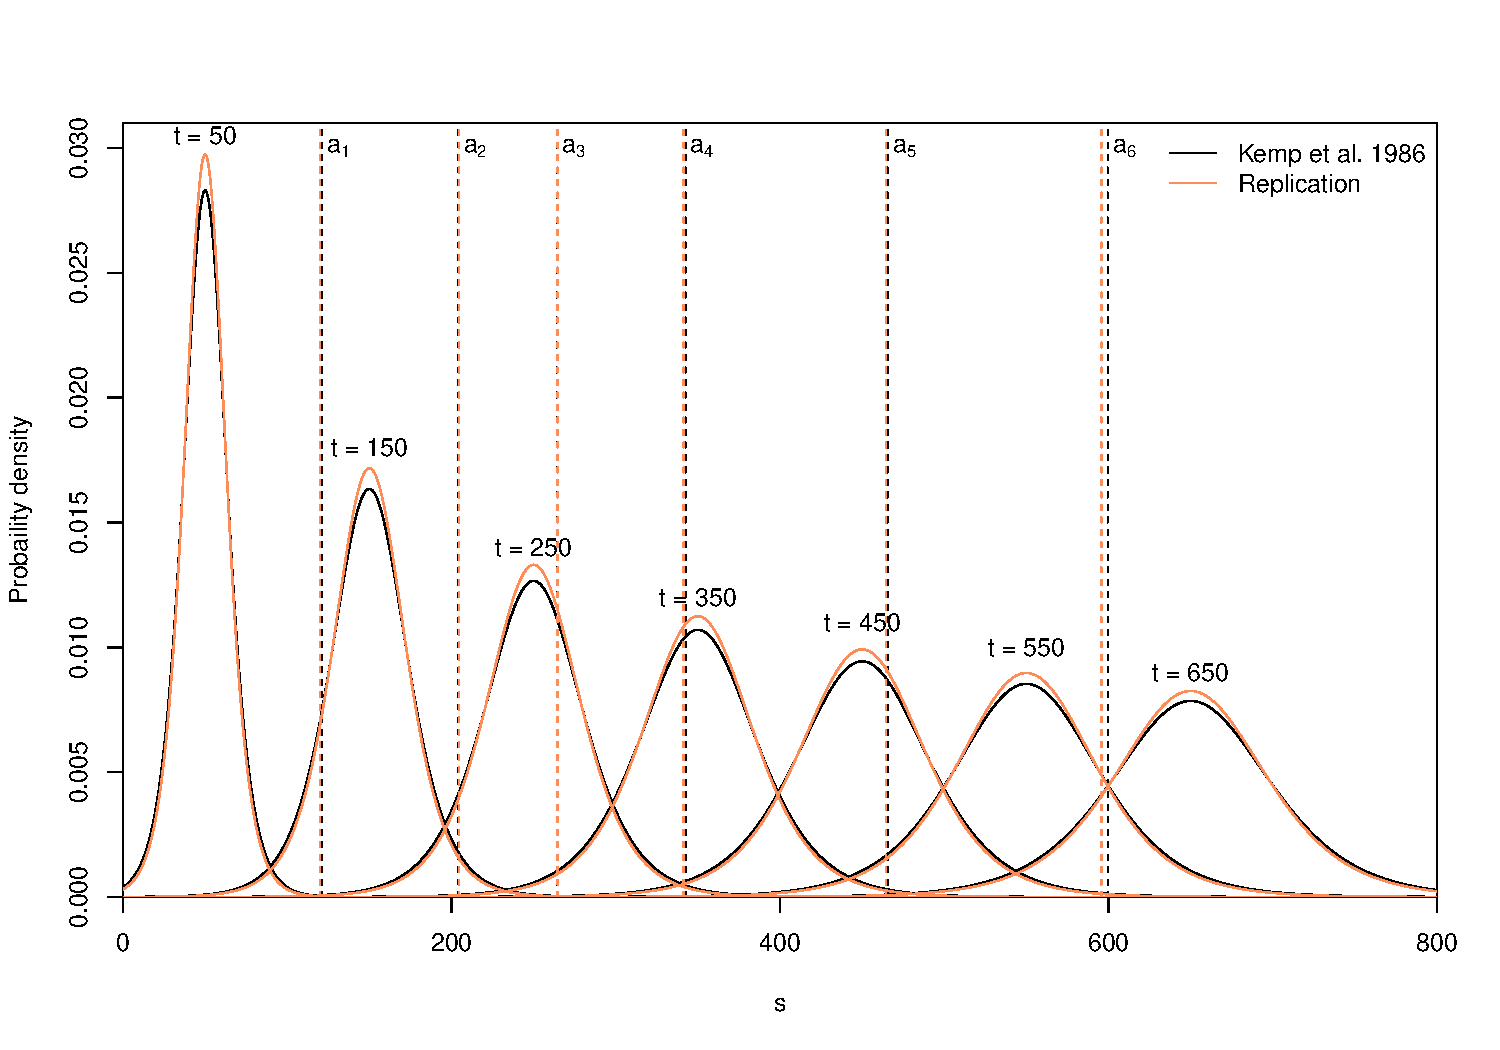
\includegraphics[width=\textwidth]{../figures/dennis_fig2.pdf}
  \caption{Logistic PDF of the \citet{dennis1986stochastic} model plotted for seven fixed values of~$t$. Area under the PDF between $a_{j-1}$ and $a_j$ gives the expected proportion of insects in stage $j$ at time $t$. Values of $a_j$ and $b^2$ used in the graph are the estimates given in Table 1 of \citep{kemp1986stochastic} (black lines) and the estimates from the replication (red lines). This figure replicates Figure 2 in \citep{dennis1986stochastic}.}
  \label{fig:fig1}
\end{figure}

\section{Results}
\begin{figure}[p]
  \centering
  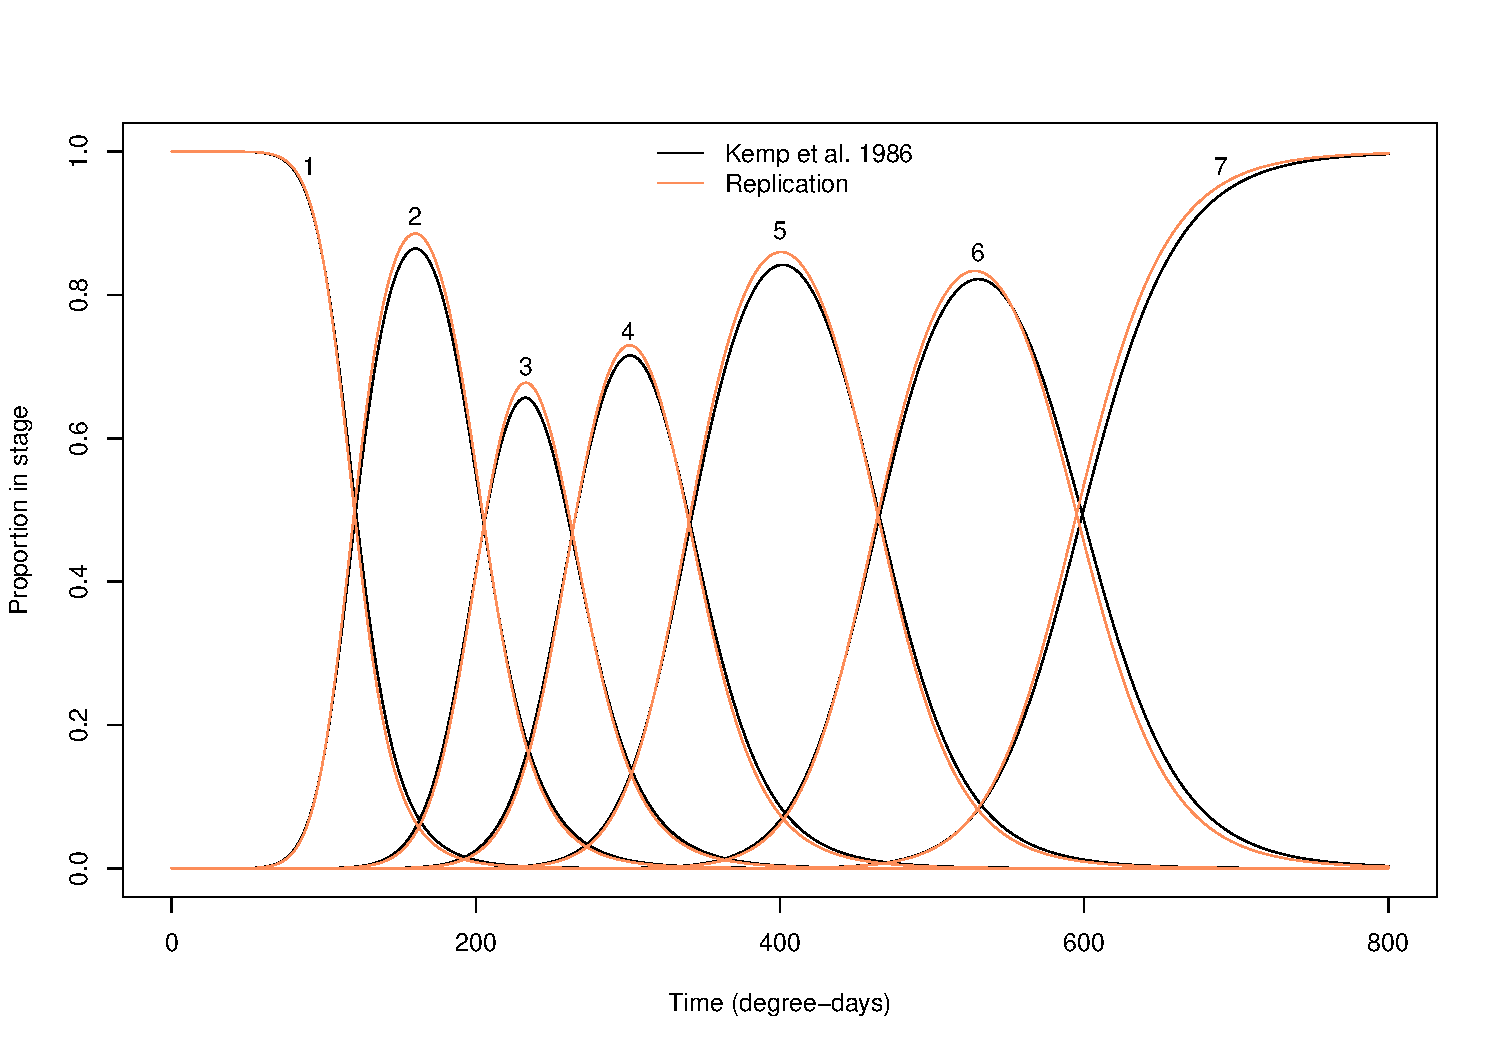
\includegraphics[width=\textwidth]{../figures/dennis_fig3.pdf}
  \caption{Expected proportion of insects in stages 1-7 plotted as functions of time $t$. Values of $a_j$ and $b^2$ used in the graph are the estimates given in Table 1 of \citep{kemp1986stochastic} (black lines) and the estimates from the replication (red lines). This figure replicates Figure 3 in \citep{dennis1986stochastic}.}
  \label{fig:fig2}
\end{figure}

\subsection{Sequential model}

\begin{table}
  \small
    \centering
    \caption{Parameter estimates for the sequential model with stopping ratios. This table replicates results presented in Table~3 of \citep{candy1991modeling}.}
  
\begin{tabular}{lrrrrrrll}
\toprule
Parameter & $\beta_{\_1}$ & $\beta_{\_2}$ & $\beta_{\_3}$ & $\beta_{\_4}$ & $\beta_{\_5}$ & $\beta_{\_6}$ & Link & Method\\
\midrule
$\beta_{0j}$ & 10.410 & 12.960 & 12.020 & 11.160 & 17.700 & 33.730 & logit & Original \citep{candy1991modeling}\\
$\beta_{0j}$ & 10.410 & 12.959 & 12.020 & 11.165 & 17.698 & 33.726 & logit & R \verb+vglm+\\
$\beta_{1j}$ & -0.085 & -0.062 & -0.046 & -0.033 & -0.038 & -0.056 & logit & Original \citep{candy1991modeling}\\
$\beta_{1j}$ & -0.085 & -0.062 & -0.046 & -0.033 & -0.038 & -0.056 & logit & R \verb+vglm+\\
\addlinespace
$\beta_{0j}$ & 7.350 & 8.530 & 9.120 & 8.440 & 10.090 & 16.300 & cloglog & Original \citep{candy1991modeling}\\
$\beta_{0j}$ & NA & NA & NA & NA & NA & NA & cloglog & R \verb+vglm+\\
$\beta_{1j}$ & -0.065 & -0.044 & -0.037 & -0.026 & -0.023 & -0.029 & cloglog & Original \citep{candy1991modeling}\\
$\beta_{1j}$ & NA & NA & NA & NA & NA & NA & cloglog & R \verb+vglm+\\
\bottomrule
\end{tabular}
  \label{tab:tab3}
\end{table}

